\documentclass[border=4pt]{standalone}
\usepackage{amsmath,amssymb,tikz}
\usetikzlibrary{arrows.meta,calc}
\definecolor{figB}{RGB}{31,90,166}\definecolor{figR}{RGB}{176,48,48}\definecolor{figG}{RGB}{46,125,50}\definecolor{figO}{RGB}{214,120,20}
\begin{document}
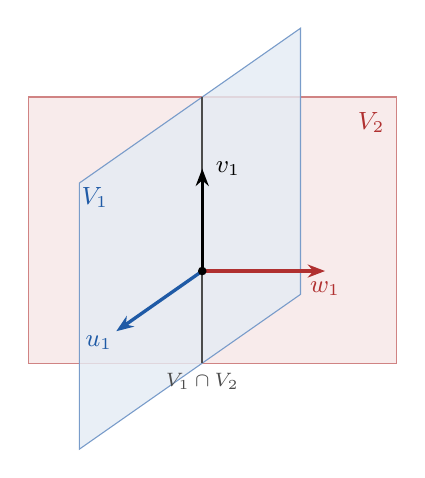
\begin{tikzpicture}[scale=1.3,>={Stealth[length=2.2mm]},x={(-0.6cm,-0.42cm)},y={(1cm,0cm)},z={(0cm,1cm)}]
% V2 = yz-plane (back wall), V1 = xz-plane
\fill[figR!12,fill opacity=0.8] (0,-1.7,-0.9)--(0,1.9,-0.9)--(0,1.9,1.7)--(0,-1.7,1.7)--cycle;
\draw[figR!60] (0,-1.7,-0.9)--(0,1.9,-0.9)--(0,1.9,1.7)--(0,-1.7,1.7)--cycle;
\fill[figB!12,fill opacity=0.8] (-1.6,0,-0.9)--(2.0,0,-0.9)--(2.0,0,1.7)--(-1.6,0,1.7)--cycle;
\draw[figB!60] (-1.6,0,-0.9)--(2.0,0,-0.9)--(2.0,0,1.7)--(-1.6,0,1.7)--cycle;
\draw[black!70,thick] (0,0,1.7)--(0,0,-0.9) node[below,font=\scriptsize]{$V_1\cap V_2$};
\node[figB,font=\small] at (1.75,0,1.45) {$V_1$};
\node[figR,font=\small] at (0,1.65,1.45) {$V_2$};
\draw[->,very thick] (0,0,0)--(0,0,1) node[right,font=\small,xshift=1pt]{$v_1$};
\draw[->,very thick,figB] (0,0,0)--(1.4,0,0) node[below left,font=\small,inner sep=1pt]{$u_1$};
\draw[->,very thick,figR] (0,0,0)--(0,1.2,0) node[below,font=\small]{$w_1$};
\fill (0,0,0) circle (1.2pt);
\end{tikzpicture}
\end{document}
